\section{Рабочий проект}
\subsection{Классы, используемые при разработке системы управления энергопотреблением}

В процессе разработки системы управления энергопотреблением были использованы различные классы для обеспечения функциональности и взаимодействия компонентов. Ниже представлен список ключевых классов и их методов, применяемых в разрабатываемой программной системе (таблица \ref{class:table_energy_management}).

\renewcommand{\arraystretch}{0.8} % уменьшение расстояний до сетки таблицы
\begin{xltabular}{\textwidth}{|X|p{2.5cm}|>{\setlength{\baselineskip}{0.7\baselineskip}}p{4.85cm}|>{\setlength{\baselineskip}{0.7\baselineskip}}p{4.85cm}|}
	\caption{Описание классов системы управления энергопотреблением\label{class:table_energy_management}}\\
	\hline \centrow \setlength{\baselineskip}{0.7\baselineskip} Название класса & \centrow \setlength{\baselineskip}{0.7\baselineskip} Модуль, к которому относится класс & \centrow Описание класса & \centrow Методы \\ \hline
	
	\endfirsthead
	
	\caption*{Продолжение таблицы \ref{class:table_energy_management}}\\  
	\hline \centrow \setlength{\baselineskip}{0.7\baselineskip} Название класса & \centrow \setlength{\baselineskip}{0.7\baselineskip} Модуль, к которому относится класс & \centrow Описание класса & \centrow Методы \\  \hline
	
	\finishhead
	
	Energy Consumption & Models & Класс, отвечающий за учет и хранение данных о потреблении энергии в зданиях. Атрибуты класса включают в себя информацию о компании, помещении, этаже, дате, количестве потребленной энергии с и без использования системы управления, общей стоимости, а также дополнительные параметры, такие как влажность, температура, освещенность и обнаружение движения. &  Метод \_\_str\_\_ обеспечивает читаемое представление объекта этого класса. \\
	\hline
	
	Inventory Items Number & Models & Класс, предназначенный для представления предметов, находящихся в конкретном помещении. Атрибуты класса включают в себя название предмета и ссылку на помещение, где он находится.  & Метод \_\_str\_\_ обеспечивает читаемое представление объекта этого класса. \\
	\hline
	
	Company & Models & Класс, используемый для представления компаний, использующих систему управления энергопотреблением. Атрибуты класса включают в себя название компании, цвет для визуализации, тип объекта компании и количество сотрудников. &  Метод \_\_str\_\_ обеспечивает читаемое представление объекта этого класса. \\
	\hline
	
	Floor & Models & Класс, предназначен для представления этажей. & Метод \_\_str\_\_ обеспечивает читаемое представление объекта этого класса. \\
	\hline
	
	Electricity & Models & Класс, используемый для представления электроэнергии, собираемой и потребляемой системой. Атрибуты класса включают в себя цену за единицу электроэнергии и объем потребленной энергии. &  Метод \_\_str\_\_ обеспечивает читаемое представление объекта этого класса. \\
	\hline
	
	Inventory Items & Models & Класс, представляющий предметы инвентаря. Атрибуты включают в себя наименование предмета и потребление энергии в кВт·ч. &  Метод \_\_str\_\_ обеспечивает читаемое представление объекта этого класса. \\
	\hline

	Address & Models & Класс, представляющий адрес объекта. Атрибуты включают в себя город, улицу, номер дома и строение. &  Метод \_\_str\_\_ обеспечивает читаемое представление объекта этого класса. \\
	\hline
	
	Street & Models & Класс, представляющий улицы. Атрибут включает в себя название улицы. &  Метод \_\_str\_\_ обеспечивает читаемое представление объекта этого класса. \\
	\hline
	
	City & Models & Класс, представляющий города. Атрибут включает в себя название города. &  Метод \_\_str\_\_ обеспечивает читаемое представление объекта этого класса. \\
	
\end{xltabular}
\renewcommand{\arraystretch}{1.0} % восстановление сетки



\subsection{Модульное тестирование разработанной системы управления энергопотреблением}


Для обеспечения надежности и корректности работы класса EnergyConsumption в приложении, был разработан и реализован модульный тест. Этот тест написан с использованием фреймворка тестирования Django и охватывает различные аспекты функционала класса.

Описание теста:

1. Настройка среды тестирования:
- Создание тестового объекта EnergyConsumption.
- Установка значений полей объекта для проведения тестов.

2. Проверка метода \_\_str\_\_:
- Вызов метода \_\_str\_\_ для объекта EnergyConsumption.
- Сравнение возвращаемой строки с ожидаемым результатом.
- Ожидается, что строка содержит информацию о компании, комнате и дате.

3. Ожидаемые результаты:
- Успешное создание и сохранение объекта EnergyConsumption.
- Корректное функционирование метода \_\_str\_\_ с возвращением ожидаемой строки.
- Этот модульный тест помогает обеспечить стабильность и правильную работу класса EnergyConsumption, а также может быть использован при внесении изменений в код для подтверждения его надежности.


Модульное тестирование класса EnergyConsumption представлен на рисунке \ref{EnergyConsumption:image}.
\begin{figure}[ht]
	\begin{lstlisting}[language=Python]
		from django.test import TestCase
		from .models import EnergyConsumption
		
		class EnergyConsumptionTestCase(TestCase):
			def setUp(self):
				self.energy_consumption = EnergyConsumption(
				company_name='Test Company',
				room='Test Room',
				floor='Test Floor',
				date='2023-01-01',
				consumption_without_an_assistant={'value': 100, 'unit': 'kWh'},
				consumption_with_an_assistant={'value': 80, 'unit': 'kWh'},
				total_amount_of_electricity_consumed_without_an_assistant=100,
				total_amount_of_electricity_consumed_with_the_assistant=80,
				total_cost_without_an_assistant={'value': 100, 'currency': 'USD'},
				total_cost_with_an_assistant={'value': 80, 'currency': 'USD'},
				humidity={'value': 50, 'unit': '%'},
				temperature={'value': 25, 'unit': 'C'},
				illumination={'value': 500, 'unit': 'lux'},
				motion={'value': True}
				)
				self.energy_consumption.save()
				
			def test_energy_consumption_str_method(self):
				# Проверяем, что метод __str__ возвращает ожидаемую строку
				expected_str = 'Компания: Test Company|Test Room, Дата: 2023-01-01'
				self.assertEqual(str(self.energy_consumption), expected_str)
				
	\end{lstlisting}  
	
	\caption{Модульный тест класса EnergyConsumption}
	\label{EnergyConsumption:image}
\end{figure}

\newpage

Для обеспечения корректной работы и надежности функционала класса Company, был разработан модульный тест, использующий фреймворк тестирования Django.

Описание теста:

1. Настройка среды тестирования:
- Создание тестового объекта Company.
- Установка значений полей объекта для проведения тестов.

2. Проверка метода \_\_str\_\_:
- Вызов метода \_\_str\_\_ для объекта Company.
- Сравнение возвращаемой строки с ожидаемым результатом.
- Ожидается, что строка содержит информацию о названии компании.

3. Проверка метода save:
- Сохранение объекта Company в базе данных.
- Попытка извлечения сохраненного объекта из базы данных.
- Сравнение извлеченного объекта с исходным для подтверждения сохранения в базе.

Ожидаемые результаты:
- Успешное создание и сохранение объекта Company.
- Корректное функционирование метода \_\_str\_\_ с возвращением ожидаемой строки.
- Успешное сохранение объекта в базе данных и его последующее извлечение.

Модульное тестирование класса Company представлен на рисунке \ref{Company:image}.

\begin{figure}[ht]
\begin{lstlisting}[language=Python]

from django.test import TestCase
from .models import Company

class CompanyTestCase(TestCase):

	def setUp(self):
		# Создаем тестовый объект Company
		self.company = Company(
		name='Test Company',
		color='Test Color',
		object='Test Object',
		number_of_employees='50'
		)
		self.company.save()
	
	def test_company_str_method(self):
		# Проверяем, что метод __str__ возвращает ожидаемую строку
		expected_str = 'Test Company'
		self.assertEqual(str(self.company), expected_str)

\end{lstlisting}  
\caption{Модульный тест класса EnergyConsumption}
\label{Company:image}
\end{figure}


\newpage

Для обеспечения корректной работы и надежности функционала класса InventoryItemsNumber, был разработан модульный тест.

Описание теста:

1. Настройка среды тестирования:
- Создание тестового объекта InventoryItemsNumber.
- Установка значений полей объекта для проведения тестов.

2. Проверка метода \_\_str\_\_:
- Вызов метода \_\_str\_\_ для объекта InventoryItemsNumber.
- Сравнение возвращаемой строки с ожидаемым результатом.
- Ожидается, что строка содержит информацию о номере инвентаря.

3. Проверка метода save:
- Сохранение объекта InventoryItemsNumber в базе данных.
- Попытка извлечения сохраненного объекта из базы данных.
- Сравнение извлеченного объекта с исходным для сохранения в базе.

Ожидаемые результаты:
- Успешное создание и сохранение объекта InventoryItemsNumber.
- Корректное функционирование метода \_\_str\_\_ с возвращением ожидаемой строки.
- Успешное сохранение объекта в базе данных и его последующее извлечение.

Модульное тестирование класса InventoryItemsNumber представлен на рисунке \ref{InventoryItemsNumber:image}.

\begin{figure}[ht]
\begin{lstlisting}[language=Python]		
from django.test import TestCase
from .models import InventoryItemsNumber 

class InventoryItemsNumberTestCase(TestCase):
	def setUp(self):
		# Создаем тестовый объект InventoryItemsNumber
		self.inventory_item_number = InventoryItemsNumber(
		name='Test Item',
		room='Test Room'
		)
		self.inventory_item_number.save()
	def test_inventory_item_number_str_method(self):
		# Проверяем, что метод __str__ возвращает ожидаемую строку
		expected_str = 'Test Item, Test Room'
		self.assertEqual(str(self.inventory_item_number), expected_str)

\end{lstlisting}  
\caption{Модульный тест класса InventoryItemsNumber}
\label{InventoryItemsNumber:image}
\end{figure}

\newpage

Для обеспечения корректной работы и надежности функционала класса Floor, был разработан модульный тест, использующий фреймворк тестирования Django.

Описание теста:

1. Настройка среды тестирования:
- Создание тестового объекта Floor.
- Установка значений полей объекта для проведения тестов.

2. Проверка метода \_\_str\_\_:
- Вызов метода \_\_str\_\_ для объекта Floor.
- Сравнение возвращаемой строки с ожидаемым результатом.
- Ожидается, что строка содержит информацию о номере этажа.

3. Проверка метода save:
- Сохранение объекта Floor в базе данных.
- Попытка извлечения сохраненного объекта из базы данных.
- Сравнение извлеченного объекта с исходным для подтверждения сохранения в базе.

Ожидаемые результаты:
- Успешное создание и сохранение объекта Floor.
- Корректное функционирование метода \_\_str\_\_ с возвращением ожидаемой строки.
- Успешное сохранение объекта в базе данных и его последующее извлечение.

Модульное тестирование класса Floor представлен на рисунке \ref{Floor:image}.


\begin{figure}[ht]
\begin{lstlisting}[language=Python]
from django.test import TestCase
from .models import Floor

class FloorTestCase(TestCase):

	def setUp(self):
		# Создаем тестовый объект Floor
		self.floor = Floor(
		number='Test Number'
		)
		self.floor.save()
	
	def test_floor_str_method(self):
		# Проверяем, что метод __str__ возвращает ожидаемую строку
		expected_str = 'Этаж Test Number'
		self.assertEqual(str(self.floor), expected_str)


\end{lstlisting}  
\caption{Модульный тест класса Floor}
\label{Floor:image}
\end{figure}

\newpage

Для обеспечения корректной работы и надежности функционала класса Electricity, был разработан модульный тест, использующий фреймворк тестирования Django.

Описание теста:

1. Настройка среды тестирования:
- Создание тестового объекта Electricity.
- Установка значений полей объекта для проведения тестов.

2. Проверка метода \_\_str\_\_:
- Вызов метода \_\_str\_\_ для объекта Electricity.
- Сравнение возвращаемой строки с ожидаемым результатом.
- Ожидается, что строка содержит информацию о потреблении электроэнергии.

3. Проверка метода save:
- Сохранение объекта Electricity в базе данных.
- Попытка извлечения сохраненного объекта из базы данных.
- Сравнение извлеченного объекта с исходным для подтверждения сохранения в базе.

Ожидаемые результаты:
- Успешное создание и сохранение объекта Electricity.
- Корректное функционирование метода \_\_str\_\_ с возвращением ожидаемой строки.
- Успешное сохранение объекта в базе данных и его последующее извлечение.

Модульное тестирование класса Electricity представлен на рисунке \ref{Electricity:image}.

\begin{figure}[ht]
\begin{lstlisting}[language=Python]
from django.test import TestCase
from .models import Electricity
	
class ElectricityTestCase(TestCase):

	def setUp(self):
		# Создаем тестовый объект Electricity
		self.electricity = Electricity(
		price=0.15,
		volume='100 kWh'
		)
		self.electricity.save()
	
	def test_electricity_str_method(self):
		# Проверяем, что метод __str__ возвращает ожидаемую строку
		expected_str = 'Цена за 100 kWh: 0.15 руб.'
		self.assertEqual(str(self.electricity), expected_str)

\end{lstlisting}  
\caption{Модульный тест класса Electricity}
\label{Electricity:image}
\end{figure}

\newpage


\subsection{Системное тестирование разработанного web-сайта}


На рисунках  ~\ref{templ11:image} - ~\ref{templ21:image} представлена главная страница  «Программно-информационной системы для управления энергопотреблением в зданиях».

Страница с аналитикой энергопотребления в здании представлена на рисунках


\begin{figure}[ht] % H - рисунок обязательно здесь, или переносится, оставляя пустоту
\center{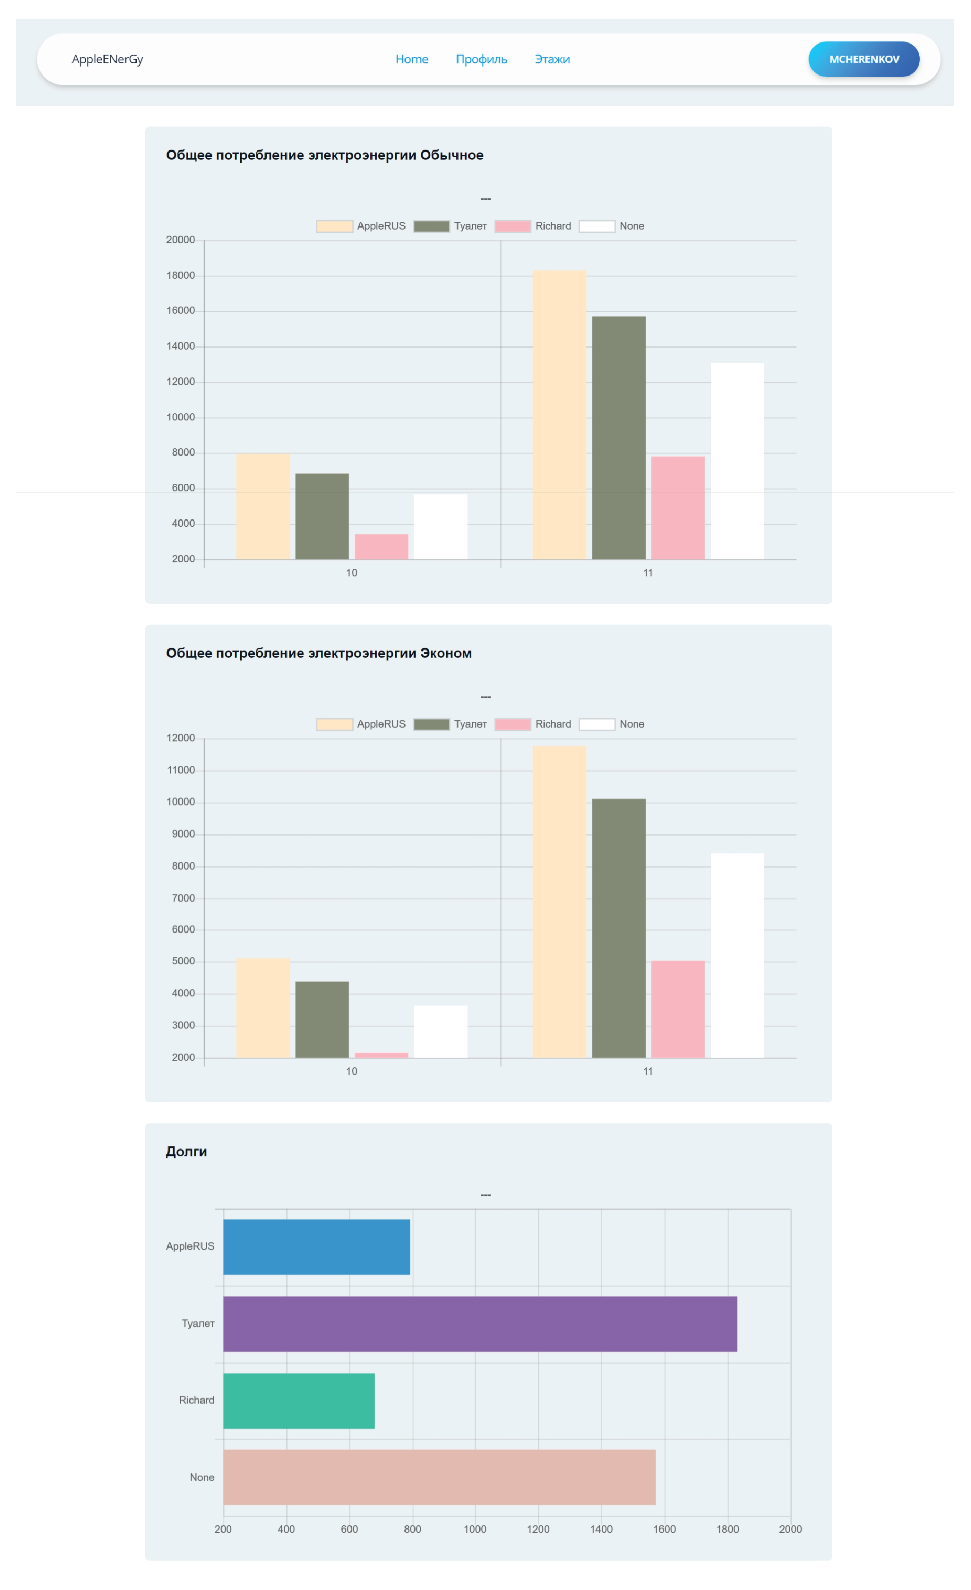
\includegraphics[width=0.6\linewidth]{templ1}}
\caption{главная страница  «Программно-информационной системы для управления энергопотреблением в зданиях»}
\label{templ11:image}
\end{figure}

\begin{figure}[H] % H - рисунок обязательно здесь, или переносится, оставляя пустоту
\center{\includegraphics[width=0.75\linewidth]{templ2}}
\caption{главная страница  «Программно-информационной системы для управления энергопотреблением в зданиях»}
\label{templ21:image}
\end{figure}

\newpage

На изображении, представленном на рисунке \ref{main1:image}, приведен план этажа, на котором наглядно отображено размещение помещений.
 

\begin{figure}[ht]
\center{\includegraphics[width=0.8\linewidth]{main1}}
\caption{План этажа}
\label{main1:image}
\end{figure}

На рисунке \ref{main2:image} изображено помещение компании.

\begin{figure}[ht]
\center{\includegraphics[width=0.8\linewidth]{main2}}
\caption{Помещение компании}
\label{main2:image}
\end{figure}

На рисунках \ref{main3:image} - \ref{main4:image}представлена диаграмма, отражающая потребление электроэнергии, температуру, влажность, освещенность, а также обнаружение движения в помещении компании.


\begin{landscape}
	
	\begin{figure}
		\includegraphics[width=0.82\linewidth]{main3}
		\center{Диаграмма, отражающая потребление электроэнергии, влажность в помещении компании.}
		\label{main3:image}      
	\end{figure}
	
	
		\begin{figure}
		\includegraphics[width=0.82\linewidth]{main4}
		\center{Диаграмма, отражающая температуру, освещенность, а также обнаружение движения в помещении компании.}
		\label{main4:image}      
	\end{figure}

%\begin{figure}[ht]
%	\center{\includegraphics[width=0.8\linewidth]{main3}}
%	\caption{Диаграмма, отражающая потребление электроэнергии, влажность в помещении компании.}
%	\label{main3:image}
%\end{figure}


%\begin{figure}[ht]
%	\center{\includegraphics[width=0.8\linewidth]{main4}}
%	\caption{Диаграмма, отражающая температуру, освещенность, а также обнаружение движения в помещении компании.}
%	\label{main4:image}
%\end{figure}

\end{landscape}

\newpage